\documentclass[11pt,a4paper]{article}
\usepackage[utf8]{inputenc}
\usepackage{graphicx}
\usepackage{blindtext}
\usepackage{amsmath}
\usepackage{amssymb}
\usepackage{mathpazo}
%\usepackage{gensymb} % gives an error
\usepackage{caption}
\usepackage[toc,page]{appendix} % needed for appendices
\usepackage{enumitem}
\usepackage{hyperref}
\usepackage{wrapfig}
\usepackage{colortbl} % needed for coloured columns in appendix
\usepackage{svg}
\usepackage{subfig}
\usepackage{gensymb}
\usepackage[parfill]{parskip}%https://tex.stackexchange.com/questions/40429/how-to-use-the-parskip-package-space-in-between-paragraphs

\usepackage[a4paper,left=1.9cm,right=1.32cm,top=1.9cm,bottom=3.67cm]{geometry}

\begin{document}
\begin{titlepage}
	\newcommand{\HRule}{\rule{\linewidth}{0.5mm}} 
	\center	
	\textsc{\LARGE University of Twente}\\[1cm] 
	\textsc{\large Mechanical Engineering}\\[0.5cm] \HRule\\[0.4cm]
	{\huge\bfseries Design of a 4 DOF high accuracy non-contact measurement probe}\\[0.4cm] 
	\HRule\\[1.5cm]
		\textsc{\large Design Principles for Precision Mechanisms }\\[0.5cm] 
    
\noindent \textit{Written by} \\
M.R.G. \textsc{Hemsteede} - s1741306\\
F.W. \textsc{Schermer} - s1723413 \\
C. \textsc{van Boggelen} - s1691297 \\
M.T. \textsc{Hop} - s1725092 \\
F. \textsc{Emming} - s1600753

\vfill\vfill\vfill
	{\large\today} \vfill 
	\end{titlepage}

\tableofcontents
\setcounter{page}{0}
\newpage
\section{Introduction}

In the "Design Principles for Precision Mechanisms II" course a project has to be made. The project is provided by DEMCON, a spin off of the University of Twente. DEMCON is a company which develops and produces systems, with as focus areas high-tech, medical, optomechatronic, robotic and industrial systems $\&$ vision.

The project is based on the Nanomefos system, a 5 DOF machine which measures the form of freeform optics  of aspheric lenses. The goal is to design a miniature version of the Nanomefos which can be used in the production of lenses for smartphone cameras and small microscopes. Three types of concepts have to be developed: one concept with conventional joints, one with only flexures and a combined flexure. 

In this report first the problem is analysed in the problem statement, which is stated below, resulting in
requirements and assumptions about the problem. In the concepts part a few ideas are presented to solve
the problem. The best suitable option is chosen and further developed in the final design part.

\begin{figure}[h]
    \centering
    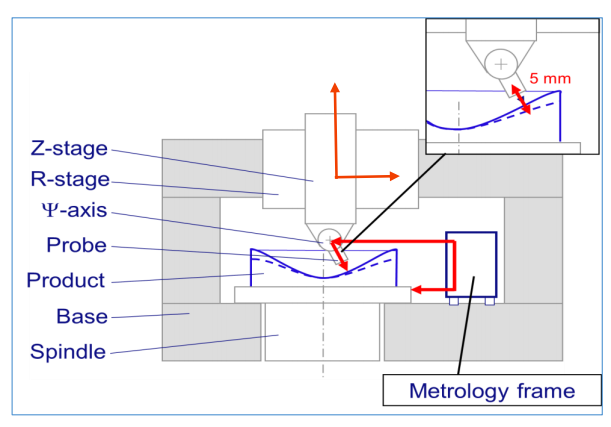
\includegraphics[width=0.6\textwidth]{images/Nanomefos.png}
    \caption{An overview of the current Nanomefos system}
    \label{fig:Nanomefos}
\end{figure}

\subsection{Problem statement}


\subsection{Requirements and Assumptions} \label{sec:requirements}
\label{requirementandassumptions}
To obtain a good design for the miniature version of the Nanomefos a number of requirements and assumptions has been made. 

\subsubsection*{Requirements}
The total mass of the probe should be $\leq 0.5\ kg$, furthermore the total space which the systems occupies has to be $\leq 300\cdot300\cdot100\ mm$.

In table \ref{tab:requirements} an overview is given of the range, duration, repeatability, velocity and acceleration for each degree of freedom. Both the range, duration and repeatability where given. Whereas the maximum velocities and accelerations are determined. 

The system has the following degrees of freedom: a translation in the x direction with a stroke of 10 mm, a translation in the z direction with a total stoke of 2 mm, a rotation around the y axis of 45 degrees and a rotation around the z axis of 90 degrees. An overview of the degrees of freedom is shown in table \ref{tab:doftable}.
\begin{table}[!h]
\centering
\caption{Required range of motion per degree of freedom}
\label{tab:doftable}
\begin{tabular}{l|llll}
Degree of Freedom & X-translation & Z-translation & Y-rotation & Z-rotation \\ \cline{1-5}
Range of motion   & 10 mm         & 2 mm          & 45 \degree  & 90 \degree 
\end{tabular}
\end{table}

\subsubsection*{Derivation of maximum velocities and accelerations}
To determine the maximum velocities and accelerations for all four degrees of freedom (X, Z, $R_y$, $R_z$), a skew sine function has been assumed for the position of the probe. This can bee seen in equation \ref{eq:skewsine}, where $h_m$ is the range of the desired displacement/rotation of the degree of freedom, while $t_m$ is the time needed to achieve this displacement/rotation.

\begin{equation} \label{eq:skewsine}
r(t)=\frac{h_m}{t_m}t-\frac{h_m}{2\pi}\sin\left(\frac{2\pi}{t_m}t\right) \\
\end{equation}

Using equation \ref{eq:skewsine}, and taking the derivative, the velocity, acceleration and jerk can be determined as seen in equation \ref{eq:skewsinederivative}. 
\begin{equation} \label{eq:skewsinederivative}
\begin{aligned}
v(t)=&r'(t)=\frac{h_m}{t_m}-\frac{h_m}{t_m}\cos\left(\frac{2\pi}{t_m}t\right) \\ 
a(t)=&r''(t)=\frac{2\pi h_m}{t_m^2}\sin\left(\frac{2\pi}{t_m}t\right) \\ 
J(t)=&r'''(t)=\frac{4\pi^2h_m}{t_m^3}\cos\left(\frac{2\pi}{t_m}t\right)
\end{aligned}
\end{equation}
The maximum velocity occurs at $a(t)=0$, while the maximum acceleration occurs at $J(T)=0$. When solving these equations for t, the time at which the maxima occur are found. Plugging this back into the original velocity and acceleration equation, the results are obtained. This can be seen in equation \ref{eq:VmaxAmax}
\begin{equation} \label{eq:VmaxAmax}
\begin{aligned}
\text{Determination of $v_{max}$} \Rightarrow \quad a(t)=0 \Rightarrow \quad t=\frac{t_m}{2} \quad \quad \quad \quad  \quad \quad & v_{max}=r'\left(\frac{t_m}{2}\right)=\frac{2h_m}{t_m} \\
\text{Determination of $a_{max}$} \Rightarrow \quad J(t)=0 \Rightarrow \quad t=\frac{t_m}{4} \quad \quad \quad \quad  \quad \quad & a_{max}=r''\left(\frac{t_m}{4}\right)=\frac{2\pi h_m}{t_m^2}
\end{aligned}
\end{equation}
Using the final expressions for the maximum velocities and accelerations, the values for all four degrees of freedom are calculated, which can be seen in table \ref{tab:requirements}.
\begin{table}[ht]
\centering
\caption{Range, duration, repeatability, velocity and acceleration per degree of freedom}
\label{tab:requirements}
\begin{tabular}{l|lllll}
\textbf{DoF} & \textbf{Range ($h_m$)}    & \textbf{Duration ($t_m$)} 	& \textbf{Repeatability} & \textbf{Velocity ($v_{max}$)} & \textbf{Acceleration ($a_{max}$)} \\ \hline
$X$                & $ \geq \pm \ 5 mm $ 		& 0.5 s 						& $\leq 1\ \mu m$         & $ 40\ mm/s $        & $  125\ mm/s^2 $                    \\
$Z$                & $ \geq \pm \ 1 mm$  		& 0.5 s						& $\leq 1\ \mu m$            &$  8\ mm/s $       &  $ 25\ mm/s^2 $                    \\
$R_y$              & $ \geq 0.785\ rad $       & 2.0 s							& $\leq 10\ \mu rad$         & $ 0.79\ rad/s$  &   $  1.23\ rad/s^2 $                \\
$R_z$              & $ \geq  1.571 \ rad $     		& 1.0	s				    & $\leq 10\ \mu rad$         & $ 3.14\ rad/s $ &   $  9.87\ rad/s^2$                 
\end{tabular}
\end{table}

\subsubsection*{Eigenfrequencies}
The internal parasitic eigenfrequency should be $\geq 200\ Hz$. To obtain the minimum lowest mechanical natural frequency the crossover frequency should be multiplied by a factor 4.

\subsubsection*{Assumptions}
To obtain a design for the miniature version of the Nanomefos a number of assumptions has been made shown in 


%\subsection{Sequence of DOF}
%As mentioned in section \ref{requirementandassumptions} there are two translational degrees of freedom and two rotational degrees of freedom. These DOF's need to be positioned in series to achieve the required range of motion. The sequence in which the DOF's are positioned in series influence the stiffness and the range of motion significantly, therefore an evaluation is done to determine the best sequence.

%\begin{wrapfigure}{r}{0.5\textwidth}
%  \begin{center}
%    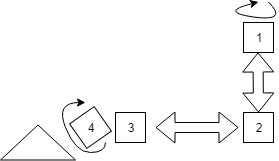
\includegraphics[width=0.4\textwidth]{images/DOF_sequence.png}
%  \end{center}
%  \caption{Sequence of DOF's}
%  \label{fig:sequencedof}
%\end{wrapfigure}

%The sequence of DOF's is visualized in figure \ref{fig:sequencedof}. Step 1 is the z-rotation of 90\degree, this has to be done first to achieve the half circle range of motion with as little required space as possible. Then in step 2 the probe is positioned at the correct height by the 2 mm of z-translation after which it is translated in the x-direction to get to its final position. As can be seen in the figure the surface of the disk is under an angle, therefore the probe will then be rotated around it's y-axis to achieve the correct orientation. 

\newpage
\section{Concept: conventional joints}
\label{Concept: conventional joints}
Three concepts are designed based on conventional joints, meaning that no flexures are used. These concepts are presented and evaluated after which one concept is selected based on a selection table.
%\subsection{Hysteresis}
%In precision products, joined parts must maintain their relative position. If under either thermal or mechanical load shift takes place most certainly the relative position in the unloaded state is also changed. The phenomenon responsible for this is hysteresis or virtual backlash. The virtual play in a simple model is described by $S_v = \frac{2W}{c}$ where $W$ is the friction and {c} the stiffness.


\subsection{Degrees of freedom}
First of all an overview is made of the different ways to enable motion in the degrees of freedom. A division is made between translational degrees of freedom and rotational degrees of freedom.
\subsubsection{Translational degrees of freedom}
As stated in section \ref{requirementandassumptions} the design has two translational degrees of freedom. In this subsection all the possibilities that a conventional design offers with regards to translational movement are evaluated. \\\\
The most common solution for translation movement is a linear bearing, these bearings exactly constrain 5 degrees of freedom and allow only translational movement. A more advanced version of the linear bearing is an H-drive. An H-drive makes use of three linear bearings which results in an increased stiffness however over-constraining the design.  \\
Another solution for translational movement uses the idea of a column press, this type of guidance is commonly used in high load application but can also be used for this application. \\
A spindle can also be used to obtain a translational movement. This option however results in a high amount of hysteresis and requires a large force to actuate. 


%\begin{enumerate}
%    \item A linear bearing. These types of bearings constraint 5 degrees of freedom and allow only translational movement. 
%    \item An H-drive, this is a commonly used linear drive in precision mechanics. 
%    \item A column press design. This design allows for only one translational degree. Usually these types of constructions are used in high load application instead of precision mechanisms.
%\end{enumerate}
\begin{table}[h] \centering \caption{Translational DOF's: solution overview} \label{tab:transsolutions}
\begin{tabular}{p{3cm}|p{3cm}p{3cm}p{3cm}p{3cm}}
Translational solution   & Linear bearing \cite{lineartrans} & H-drive \cite{lecturesheets} & Column press \cite{TOXPRESSOTECHNIK4PRESSOTECHNIK} & Spindle\\ \hline
Figure for clarification &     
    \begin{minipage}{3cm}
      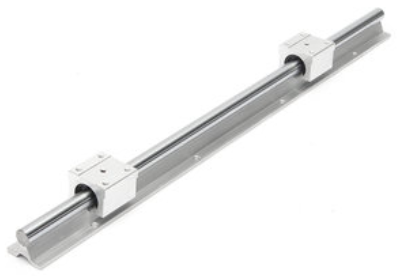
\includegraphics[width=\linewidth]{images/linear.png}
    \end{minipage} 
    &     
    \begin{minipage}{3cm}
      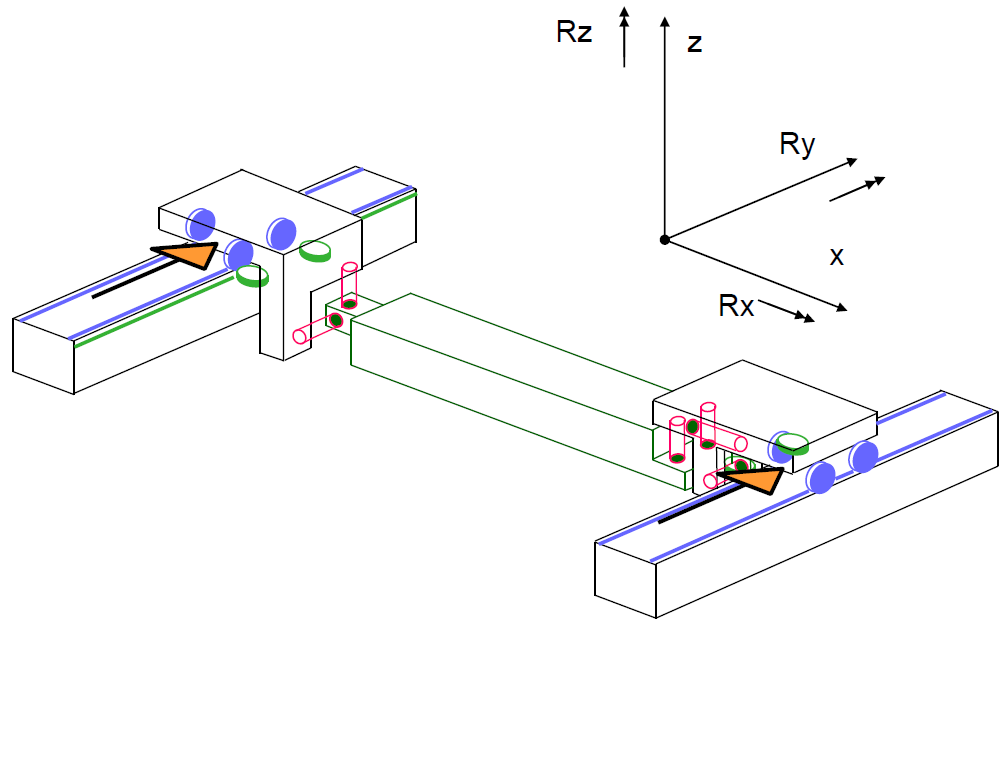
\includegraphics[width=\linewidth]{images/Hdrive}
    \end{minipage} 
    &     
    \begin{minipage}{3cm}
      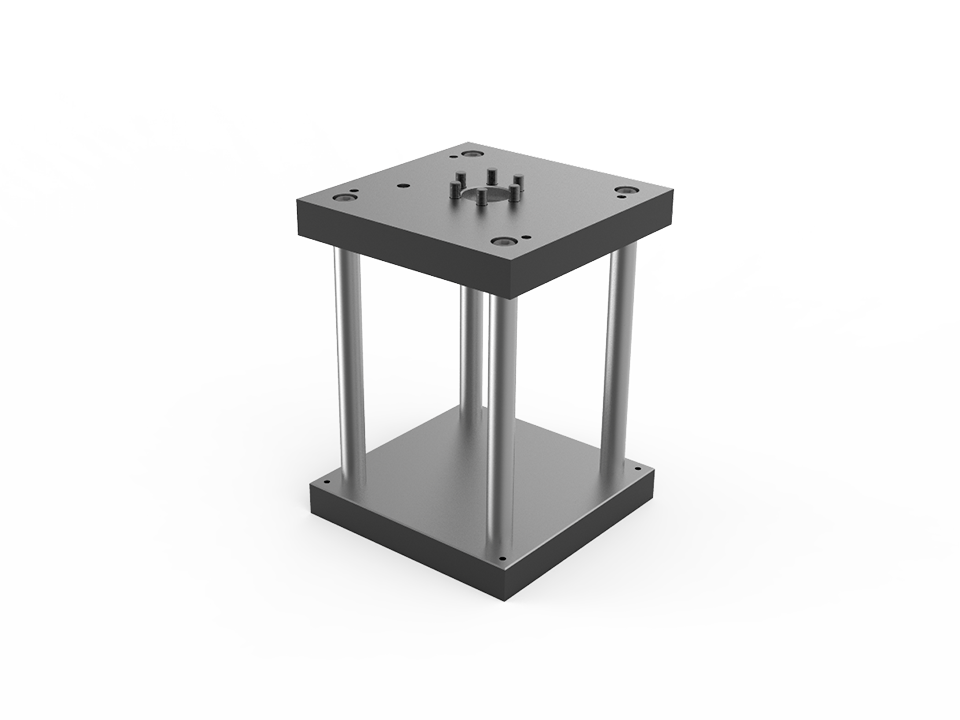
\includegraphics[width=\linewidth]{images/column_press.png}
    \end{minipage}
    &
    \begin{minipage}{3cm}
      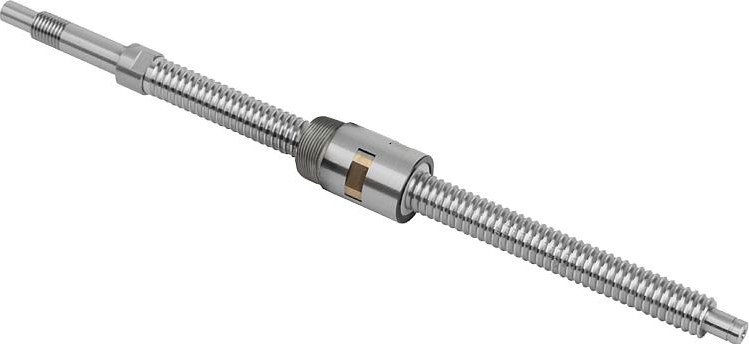
\includegraphics[width=\linewidth]{images/spindle.png}
    \end{minipage} \\ \hline
Advantages               & Exact constraint & Stiff & High loads & Relatively accurate \\ \hline
Disadvantages            & None & Vulnerable to misalignment & Over constraint & Low translational speed  \\ 
\end{tabular}
\end{table}
%\subsubsection{Selection}
%\label{translationalselection}
%Taking into account the advantages and disadvantages of the various option a selection can be made. It is clear that a column press set-up is unsuitable for the precision mechanisms application as the forces are significantly smaller than optimal and the over constrained design would require precise engineering. An h-drive setup is beneficial for application where a high stiffness is required. In the current application a conventional linear bearing is sufficient for the translation degrees of freedom.

\subsubsection{Rotational degrees of freedom}
The design requires two rotational degrees of freedom that have a range of motion of 90$^o$ as stated in section \ref{requirementandassumptions}. Non-flexure based designs have several alternatives to obtain this range of motion. \\\\
The most used solution for a rotational movement is the use of a roller bearing. Several types of roller bearings are obtainable, conventional bearing using balls, air bearings using a small film of pressurised fluid and magnetic bearings using magnetic levitation. \\
Ball joints are able to obtain both a horizontal and vertical rotation. These joints are however more difficult to actuate. \\
Another option for rotational movement is the use of a worm drive. This concept uses a worm screw in combination with a worm drive to obtain a 90 degree rotation. 
%\begin{enumerate}
%    \item A conventional roller bearing. This bearing uses two races, which are the bearing rings, between which several balls roll. These races feature grooves that are shaped such that the ball fits slightly loose. The conventional roller bearing can be further divided in radial and axial.
%    \item An air bearing, which is more advanced. These bearings use a thin film of pressurised gas instead of balls. The use of pressurised gas as interface between the two surfaces allows for a low friction bearing. Next to this lower friction air bearings also have the advantage that it allows for non contact usage, therefore neglecting problems such as friction, wear and lubricant handling. 
%    \item Magnet bearing use magnetic levitation to support the load. The rotating shaft is levitated allowing a very low friction and no mechanical wear. This type of bearing supports the highest speed of all kinds of bearings. Downside of this type is that most of the time active magnetic bearing are used, meaning that a constant input power is required. Next to this magnetic bearing tyipically require a back-up bearing in the case of power or control system failure. 
%\end{enumerate}

\begin{table}[h] \centering \caption{Rotational DOF's: solution overview} \label{tab:rotationsolutions}
\begin{tabular}{p{4cm}|p{4cm}p{4cm}p{4cm}}
Rotational solution         & Roller bearing \cite{123RFBall54180420.} & Air bearing \cite{NELSONAIRAirAir} & Magnetic bearing \cite{magneticbearing} \\ \hline
Figure for clarification    & 
    \begin{minipage}{4cm}
      
\includegraphics[width=\linewidth]{images/Ball_bearing2.jpg}
    \end{minipage} 
    &     
    \begin{minipage}{4cm}
      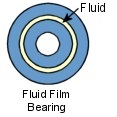
\includegraphics[width=\linewidth]{images/airbearing.jpg}
    \end{minipage} 
    &     
    \begin{minipage}{4cm}
      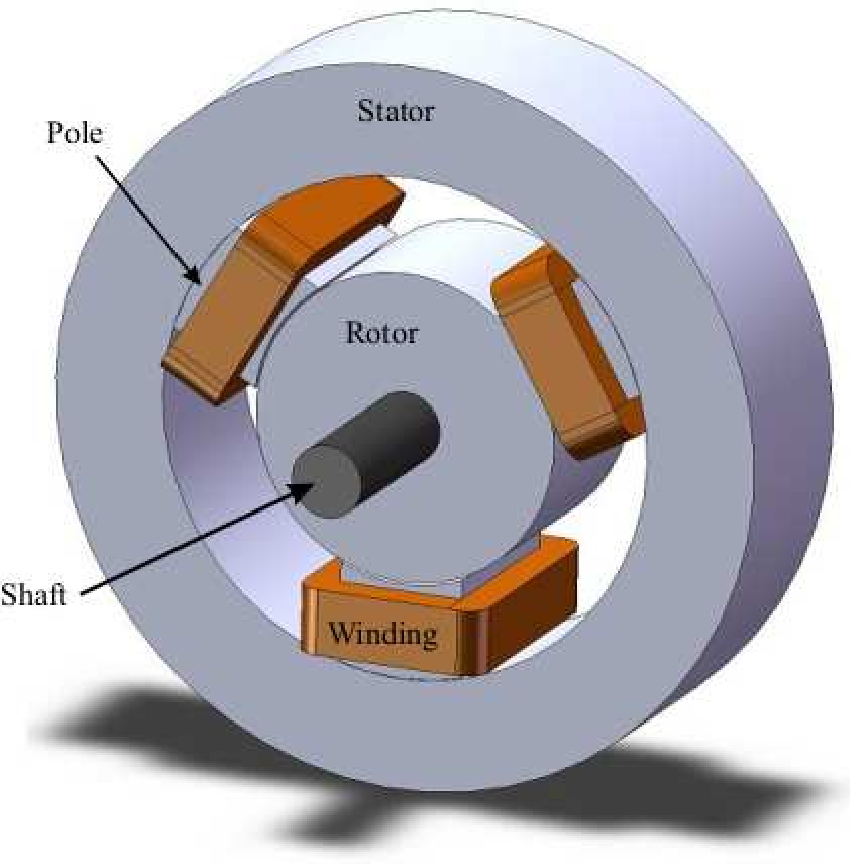
\includegraphics[width=\linewidth]{images/magnetic_bearing.png}
    \end{minipage} \\ \hline
Maximum angle               & 360\degree & 360\degree   & 360\degree  \\ \hline
Advantages                  & Cheap and widely available & Non-contact & No friction \\ \hline
Disadvantages               &  Wear and tear & Requires perfect geometry  & Large size  \\ 
\end{tabular}
\end{table}
%\subsubsection{Selection}
%\label{rotationalselection}
%Three types of bearings are proposed for the rotational degrees of freedom. The bearing will be selected based on efficiency and volume. A magnetic bearing has the lowest amount of friction however there are some drawbacks to this type, due to the required back-up bearing and constant power input the volume required for this bearing is significantly larger than the others. The available volume is limited, therefore a magnetic bearing won't be used. Roller and air bearings are both suitable for the proposed application. However due to the non-contact movement in the air bearing no wear and tear will occur which will be beneficial, therefore air bearings will be used for the rotational degrees of freedom. 

\subsection{Concept evaluation}
Knowing all the different ways to achieve the desired degrees of freedom several concepts have been made. In this section the different concepts are presented, visualised and evaluated based on several factors.
\subsubsection{Concept 1: Translational frame}
The first concept makes use of a translational table to cover the range of the disk and a double rotational cube to achieve the rotational position. This concept is shown visually in figure \ref{fig:convential_concept_1}. In this figure the translational table is shown to the left, this table makes use of several H-drive t


\begin{figure}[!h]
    \centering
    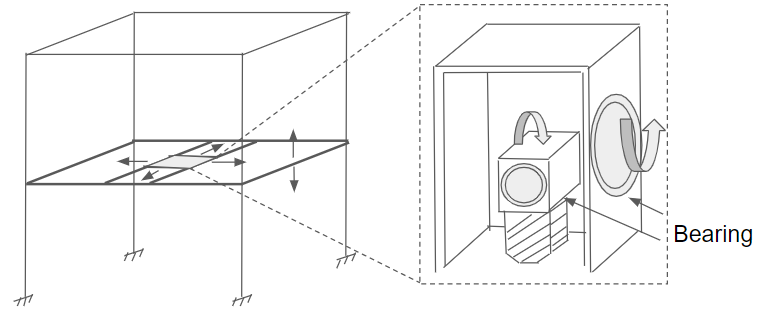
\includegraphics[width=0.6\textwidth]{images/Conventional_concept_1.PNG}
    \caption{Translational table concept}
    \label{fig:convential_concept_1}
\end{figure}



\subsubsection{Concept 2: Crane}




\subsubsection{Concept 3: Delta robot}


\subsection{Concept selection}
%As mentioned in sections \ref{rotationalselection} and \ref{translationalselection} the conventional concept will be based on linear bearings in combination with rotational air bearings. In figure \ref{fig:conventional_concept} a sketch of the concept can be seen. In this concept the first body can rotate 90 degrees, the second body can translate 1 mm, the third body can translate 10 mm and the fourth body can rotate 45 degrees. 
%\begin{figure}[h]
%    \centering
%    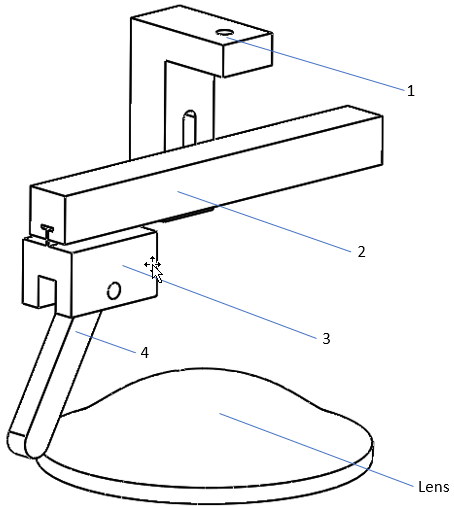
\includegraphics[width=0.5\textwidth]{images/conventional_concept.png}
%    \caption{A sketch of the conventional concept}
%    \label{fig:conventional_concept}
%\end{figure}


\newpage
\section{Concept: flexures}
\label{Concept: flexures}
The second concept is fully based on flexure mechanisms. First the options to obtain a translational motion are discussed, thereafter the solutions to obtain a rotational motion. Next three concepts are discussed and finally a concept is chosen and elaborated in more detail in section \ref{Sec: Final design}.    
\subsection{Degrees of freedom }
\subsubsection{Translational degrees of freedom}
As mentioned in section \ref{sec:requirements} the system has to have three translational degrees of freedom. In table \ref{tab:transsolutions} three options are shown to obtain a translational motion by only making use of flexures. Moreover both the advantages and disadvantages are shown.

\begin{table}[h]
\caption{Flexure based translational solutions}
\label{Tab: flexure translational}
\begin{tabular}{p{4cm}|p{4cm}p{4cm}p{4cm}}
Translational solution   & Leaf spring \cite{lecturesheets} &  \cite{PrecisionParallel} & Flexures \cite{lecturesheets} \\ \hline
Figure for clarification &     
    \begin{minipage}{4cm}
      \includegraphics[width=\linewidth]{images/}
    \end{minipage} 
    &     
    \begin{minipage}{4cm}
      \includegraphics[width=\linewidth]{images/}
    \end{minipage} 
    &     
    \begin{minipage}{4cm}
      \includegraphics[width=\linewidth]{images/}
    \end{minipage} \\ \hline
Advantages               & No parasitic motion and larger range compared to single leaf spring system     & Easier to manufacture compared to double leaf spring system  & Easy to manufacture and easy to analyse stiffness and displacement \\ \hline
Disadvantages            &  Less stiffness in the constrained direction compared to single leaf spring system                      & The system will have a parasitic motion.   & Less stiffness in direction of constrains, moreover the flexures will relative easy bend and buckle \\ 
\end{tabular}
\end{table}


\subsubsection{Rotational degrees of freedom}
Since the flexure based designs have three translational degrees of freedom the system
The design has to have two rotational degrees of freedom, one of 45$^{\circ}$ and one of 90$^{\circ}$. In this section several solutions for one rotational degree of freedom are shown.

\begin{table}[h]
\caption{Flexure based rotational solutions}
\label{Tab: flexure rotational}
\begin{tabular}{p{4cm}|p{4cm}p{4cm}p{4cm}}
Rotational solution   &  Curved flexure \cite{BrouwerELASTICDEFLECTION}   & Cross Flexure pivot \cite{Dearden2018CylindricalPivots} & Flex-16 Hinge \cite{Fowler2014Flex-16:Citation} \\ \hline
Figure for clarification &     
    \begin{minipage}{4cm}
      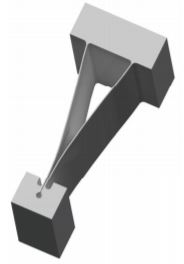
\includegraphics[width=\linewidth]{images/Cross_Brouwer.JPG}
    \end{minipage} 
    &     
    \begin{minipage}{4cm}
      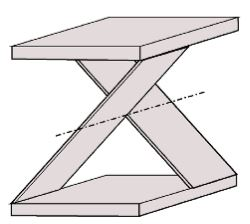
\includegraphics[width=\linewidth]{images/Cross_Flexure.JPG}
    \end{minipage} 
    &     
    \begin{minipage}{4cm}
      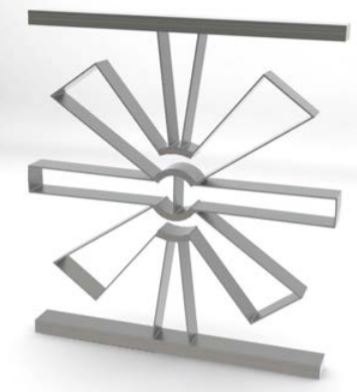
\includegraphics[width=\linewidth]{images/Flex16.JPG}
    \end{minipage} \\ \hline
Maximum rotation      & 45$^o$ &  45$^o$ & 90$^o$  \\ \hline
Advantages           &  2.5 to 14 times stiffer in stiff 
direction compared to single leaf-spring & No need of lubrication. Neither
wear nor friction occurs \cite{Haringx1949TheElement}.  & Is able to rotate 
over 90 degrees and it is a monolithic and compact design\\ \hline
Disadvantages            &  Large rotation results in limited stiffness reduction and hard to manufacture & Buckling may occur when heavily loaded, also large rotations results in a small displacement of the pivot point \cite{Haringx1949TheElement}.  & Low off-axis  stiffnesses leads to vibration problems  \\ 
\end{tabular}
\end{table}

The second concept is based on flexures, as mentioned in section \ref{requirementandassumptions} the system has four degrees of freedom, two translations and two rotations. 

To obtain a rotation of 45 degrees around the y axis, a cross-axis flexural pivot is used. Furthermore the rotation of 90 degrees around the z axis is obtained by making use of the Flex-16 hinge \cite{Fowler2014Flex-16:Citation}. Both the translations in the x and z directions are performed by double leaf spring intermediate body system, since the system has to translate over a relatively large range and has no parasitic motion. 

\subsection{Concepts evaluation}

\subsubsection{Concept A}

\subsubsection{Concept B}

\subsubsection{Concept C}

\subsection{Concept selection}
\newpage
\section{Concept: combined system}
\label{Concept: combined system}
A third concept is made based on a combination of flexures and conventional joints combining the best of both worlds.   


\subsection{Sequence of DOF's}


\subsection{Advantages and disadvantages}





\subsection{Leaf spring design}

\begin{equation}
\frac{c_{\mathrm{constr}}}{c_{\mathrm{DOF}}}>>150    
\end{equation}

\newpage
\subsection{Selection criteria}
To make a well-founded choice in the concept generation phase. Several factors are taken into account each with there own level of importance. The design consideration are listed below: 

\begin{itemize}
    \item Accuracy: The ability to reach the requirements of the stroke and repeat ability.
    \item Complexity: The complexity of the design on construction or/and control system. 
    \item Size: The requirements on the size of the machine should be met, as well as the weight of the system.
    \item Parasitic error: Unwanted movements in other direction than the actuated degree of freedom, which in term result in a lower accuracy.
    \item Velocity: Ability to meet the required velocity and sustain the acceleration.
    
\end{itemize}





\section{Decision: final concept}
\newpage
\section{Actuator choice}
Since very high accuracies have to be met, the choice of actuator(s) is of great importance as well. Not every single actuator is able to cope with such high precision. Not only does the machine have to be able to translate, it also has to be able to rotate. Therefore the actuators will be split into two categories: translational actuators and rotational actuators.
\subsection{Translational actuators}
\subsubsection*{Linear electro-mechanical (EM) actuator}
An electro-mechanical actuator is a mechanical actuator with a electric motor as control handle. Typically a mechanical actuator converts the rotary motion of the motor into translational motion. This can be done by the use of a screw for instance. Other options are belt drives, rack and pinion or other wheel and axle examples.

The advantages are that it's a relatively cheap type of actuator, and that the extending and retracting-motion behaves identically, therefore it's a pretendable type of actuator. The travel range is often quite high, while high velocity and acceleration values can be achieved. It also has a high maximum pull/push force.

The disadvantage is that it has lots of moving parts, which could wear out over time. Besides, the repeatability is often too bad compared to the requirements for this project.

\subsubsection*{Voice Coil Motor (VCM)}
Voice coil motors uses, as the name already suggests, a cylindrical coil in combination with a permanent magnet. The coil is free to move axially, which ensures the 1-directional translation. When applying a current, the end-effector is able to move quite accurately. Such a system has lots of similarities to loud-speakers for instance. A nice example can be found in \href{https://www.youtube.com/watch?v=BQJg7I-4620}{this link (click)}. 

The advantages are a that this type of actuator has zero wear, due to the air gap in between the magnet and coil. This causes hysterysis to be neglicable. Besides, it can reach high acceleration and velocity values, with a decent travel range. Also, the weight of the actuator is relatively low.  At last, there is a possibility for position feedback.

The largest disadvantage, especially in precision engineering, is the fact that VCM's do not have a perfectly linear force to travel ratio. Besides, a low mass is often required for this type of actuators, since they have to overcome the gravity.

\subsubsection*{Piezoelectric actuator}
Piezoelectric actuators make use of the special property of some materials that expand/contract when applying a voltage. This voltages can cause 1-directional movement. Very high voltages are required for small movements, which causes this type of actuator to be a short-travel-actuator.

The advantages of a piezoelectric actuator are that it can reach high acceleration values, and there is an option for long-travel actuators. Besides it consumes barely any power.

Eventhough the accelerations can be relatively high, the piezioelectric actuator cannot reach high velocities. This might not be a problem for this specific project though, since low speeds are required (see section \ref{sec:requirements}). A problem that might be of interest however, is the fact that it suffers from lots of hysterysis (due to the expanding), causing low repeatability.



\begin{table}[h] \centering \caption{Typical specifications of several translational actuator types} \label{tab:translationalactuators}
\begin{tabular}{l|cccc}
Type & Range [mm] & Repeatability [$\mu$m] & Max. vel. [mm/s] & Max. force [N] \\ \hline
EM$^{*}$            & 200 & 3 & 2000 & 123 \\
VCM$^{**}$          & 15 & 0.5 & 750 & 20 \\
Piezo$^{***}$       & 25 & 0.02 & 15 & 50 \\ \hline
Max. requirement    & 10 & $\leq 1$ & 20 & n.a.
\end{tabular}
\caption*{$^{*}$ The linear electro-mechanical actuator used for the specs is the Parker MX Miniature Positioner \cite{ElectromechanicalOverview}. \\ $^{**}$ The voice coil actuator used for specifications is the V-277 PIMag, from PI Motion Positioning \cite{V-277Actuator}. \\ $^{***}$ The piezoelectric actuator used for specifications is the PI N-331.1x PICMAWalk Walking Drive \cite{N-331Drive}.}
\end{table}





\subsection{Rotational actuators}
\subsubsection*{Stepper motors}
The Stepper motor works with a finite number of small (electro)magnets, switching on and off to move the motor in discrete steps, causing its name. Often the motor should be combined with a position encoder, so the location of the motor can be determined using impulses. 

One advantage of a stepper motor is the high rotational speeds which can be achieved. Also it can cope with a large range of loads, and often no feedback is needed since it's already combined in the motor.

However, there is a significant drop in torque at higher speeds, causing a lack of acceleration. Furthermore, the most Stepper motors have to deal with a high backlash, which causes a low accuracy. 

\subsubsection*{Servo motors}
The often used Servo motors works with an electrical (DC) motor and some kind of gearbox to reduce the rpm, while increasing torque. It is often combined with a position encoder, just as the Stepper actuator. 

The servo motors do have many advantages, for instance it has a high efficiency, can have great precision and is has an already built-in closed loop controller, which provides positional feedback. Besides, there is no torque drop at higher rotational velocities.

The biggest disadvantages is that all these advantages come with a high price tag. It is way more expensive, but also more complex and and it is more prone to errors. Besides, the actuator needs an extensive tuning before first application.

\subsubsection*{Piezoelectric actuator}
The functioning of a piezoelectric actuator has been explained in the previous paragraph, so using the material property that the material expands when a voltage is applied. The only difference is that it is in the rotational degree of freedom now.


\begin{table}[h] \centering \caption{Typical specifications of several rotational actuator types} \label{tab:rotationalactuators}
\begin{tabular}{l|cccc}
Type               & Range [rad] & Repeatability [$\mu$rad] & Vel. [rad/s] & Max. torque [Nm] \\ \hline
Stepper            & $\geq\ 2\pi$ & 1.4 & 6.283 & 6 \\
Servo              & $\geq\ 2\pi$ & 3.5 & 3.491 & 5 \\
Piezo              & $\geq\ 2\pi$ & 6.0 & 0.785 & 0.7 \\ \hline
Max. requirement   & 1.571        & $\leq 10$ & 3.14 & n.a.
\end{tabular}
\caption*{$^{*}$ The Stepper actuator used for specifications is the PI UPR-120 Ultraprecision Rotation stage \cite{UPR-120Stage}. \\ 
$^{**}$ The Servo actuator used for specifications is the PI L-611 Precision Rotation Stage \cite{L-611Stage}. \\ 
$^{***}$ The piezoelectric actuator used for specifications is the PI Q-632 Q-Motion® Rotation Stage \cite{Q-632Stage}.}
\end{table}





%\newpage
%\section{Actuator calculations}
%In order to calculate the forces needed to be achieved by the actuators, the forces in the center of gravity of the whole platform must be shifted to the point of application of the actuators. This is done by using a Jacobian 
\newpage
\section{Final design}
\label{Sec: Final design}


\subsection{Dynamics}
\newpage
\section{Conclusion}





\section{Discussion}
\newpage
\pagenumbering{gobble}
\bibliographystyle{ieeetr}
\bibliography{bronnen_handmatig.bib,michael.bib,Marvin.bib,Sjaak.bib,Casper.bib} 

\newpage
\begin{appendices} \addtocontents{toc}{\protect\setcounter{tocdepth}{0}}
\section{Bla di bla ja}
\end{appendices}

\end{document}